%\documentclass{book}
\documentclass{article}                            %for shorter notes
\usepackage{graphicx}                              %for PNG images (pdflatex)
%\usepackage{graphics}                              %for EPS images (latex)
\usepackage[linkbordercolor={1.0 1.0 0.0}]{hyperref} %for \url tag
\usepackage{color}                                 %for defining custom colours
\usepackage{framed}                                %for shaded and framed paragraphs
\usepackage{textcomp}                              %for various symbols, e.g. Registered Mark
\usepackage{geometry}                              %for defining page size
\usepackage{longtable}                             %for breaking tables
%
\geometry{verbose,a4paper,tmargin=2.5cm,bmargin=2.5cm,lmargin=2.5cm,rmargin=2cm}
\hypersetup{
  pdfauthor = {Author Name},
  pdftitle = {Paper title},
  pdfsubject = {Paper subject},
  pdfkeywords = {Paper,keyword,comma-separated},
  pdfcreator = {PDFLaTeX with hyperref package},
  pdfproducer = {PDFLaTeX}
}
%
\bibliographystyle{IEEEtran}                       %a nice bibliography style
%
\def\efill{\hfill\nopagebreak}%
\hyphenation{Nordu-Grid}
\setlength{\parindent}{0cm}
\setlength{\FrameRule}{1pt}
\setlength{\FrameSep}{8pt}
\addtolength{\parskip}{5pt}
\renewcommand{\thefootnote}{\fnsymbol{footnote}}
\renewcommand{\arraystretch}{1.3}
\newcommand{\dothis}{\colorbox{shadecolor}}
\newcommand{\globus}{Globus Toolkit\textsuperscript{\textregistered}~2~}
\newcommand{\GT}{Globus Toolkit\textsuperscript{\textregistered}}
\newcommand{\ngdl}{\url{http://ftp.nordugrid.org/download}~}
\definecolor{shadecolor}{rgb}{1,1,0.6}
\definecolor{salmon}{rgb}{1,0.9,1}
\definecolor{bordeaux}{rgb}{0.75,0.,0.}
\definecolor{cyan}{rgb}{0,1,1}
%
%----- DON'T CHANGE HEADER MATTER
\begin{document}
\def\today{\number\day/\number\month/\number\year}

\begin{titlepage}

\begin{tabular}{rl}
\resizebox*{3cm}{!}{
\includegraphics{ng-logo.png}}
&\parbox[b]{2cm}{\textbf \it {\hspace*{-1.5cm}NORDUGRID\vspace*{0.5cm}}}
\end{tabular}

\hrulefill

%-------- Change this to NORDUGRID-TECH-24

{\raggedleft NORDUGRID-TECH-24\par}

{\raggedleft \today\par}

\vspace*{2cm}

%%%%---- The title ----
{\centering \textsc{\Large Job Usage Reporter of ARC -- JURA}\Large \par}
\vspace*{0.5cm}
    
%%%%---- A subtitle, if necessary ----
{\centering \textit{\large Technical description}\large \par}
    
\vspace*{1.5cm}
%%%%---- A list of authors ----
    {\centering \large P\'eter D\'ob\'e \footnote{dobe@iit.bme.hu} \large \par}
    
%%%%---- An abstract - if style is article ----
%\begin{abstract}
%The abstract
%\end{abstract}
\end{titlepage}

%\tableofcontents                          %Comment if use article style
\newpage

\section{Introduction}

The \textit{Job Usage Reporter of ARC} (JURA) is a component
implementing a part of the accounting functionality in the ARC
middleware. Its objective is to gather metered resource usage data for
each job and submit it to accounting services along with the job
submitter's identity and miscellaneous job-related metadata.  The
collected usage data is transformed into records of job-level
granularity and a format corresponding to an OGF specification.

JURA submits the records to an accounting service.  The accounting
service stores the received usage data in a database, and provides an
interface for querying it. Queries can be made by the consumers of the
accounting data, such as a billing component. JURA is currently
capable of reporting to the logging service of the SweGrid Accounting
System (SGAS)\cite{sgas}. Maintaining the possibility to utilise other
accounting services has been kept in mind during design, the JURA
modular architecture enables easy creation of adapters for accounting
services.

JURA offers a functionality similar to that of the
\textit{logger}\cite{logger} client, with improvements and extensions.
It also serves as a complete replacement for the JARM component of
SGAS.

\section{Overview of functionality}

\begin{figure}[ht]
\centering{{{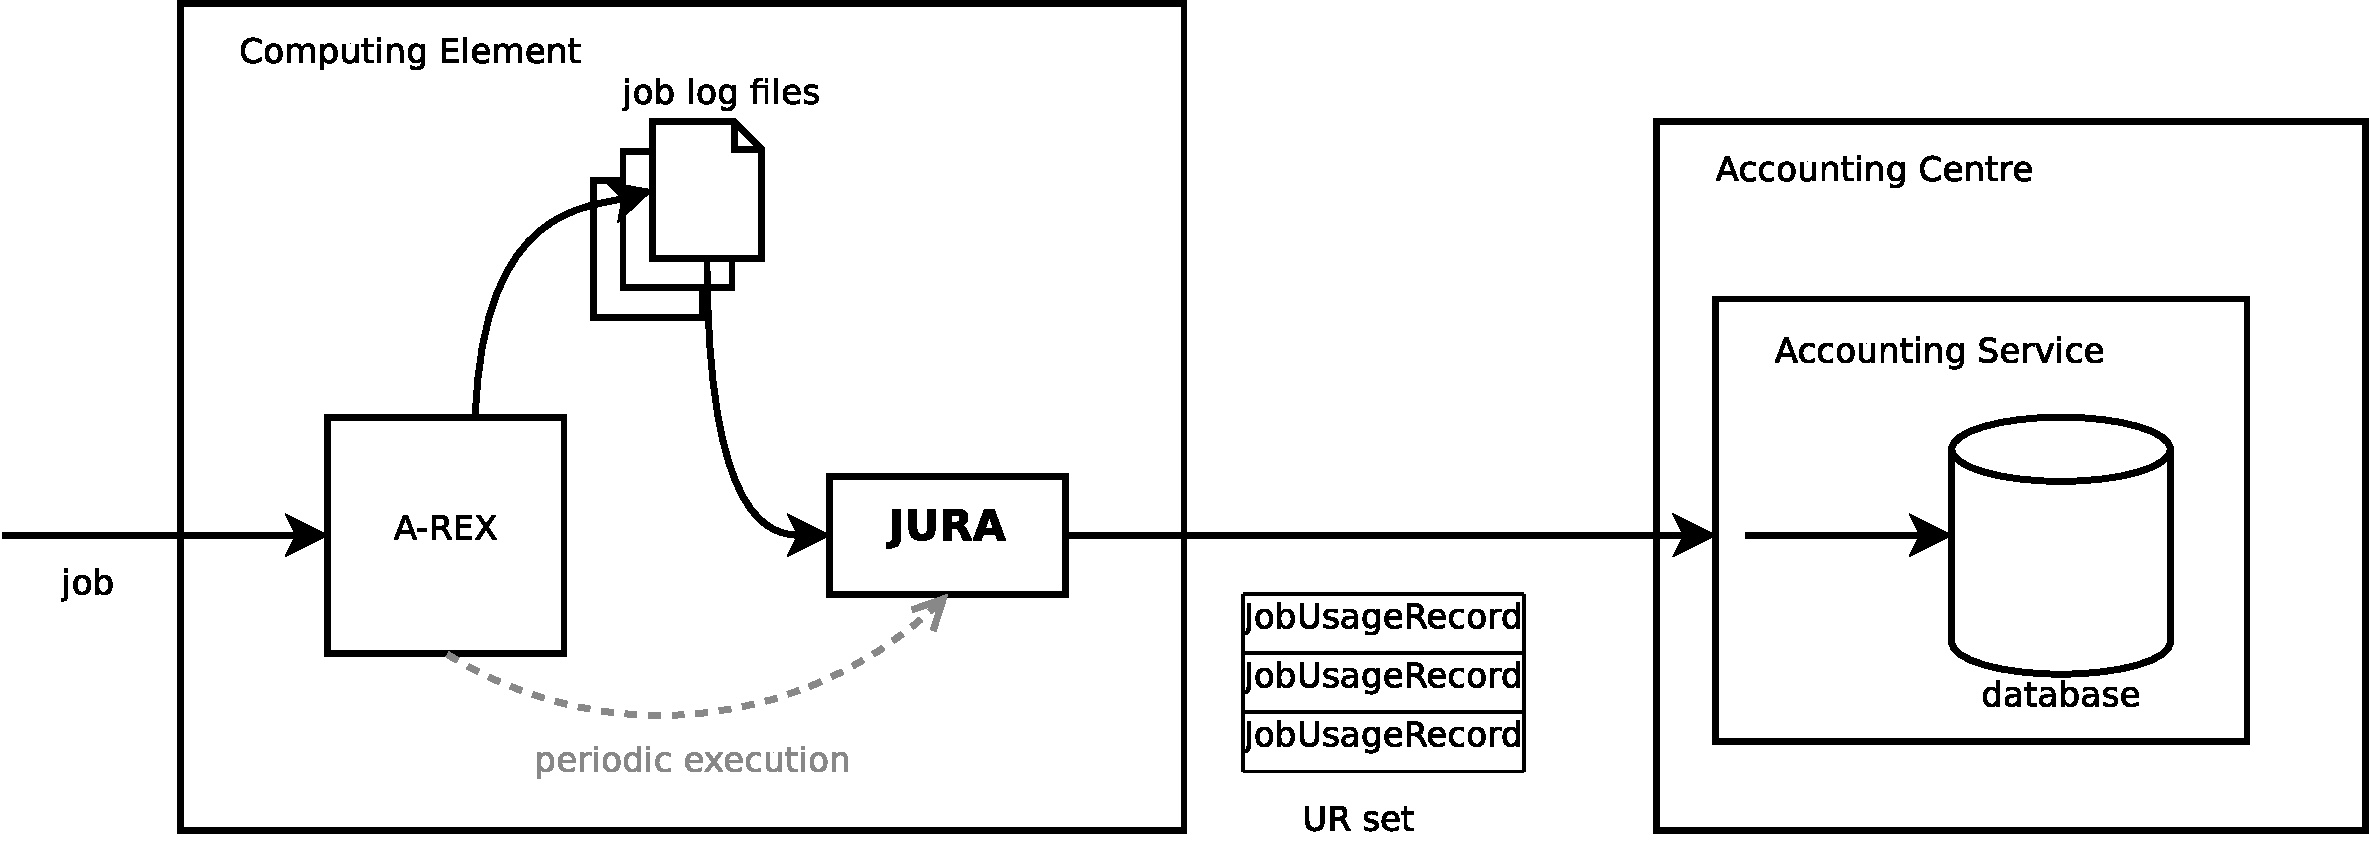
\includegraphics[width=0.9\textwidth]{components.pdf}}}
\caption{\label{fig:components}The usage reporting mechanism.} }
\end{figure}

JURA runs as a stand-alone binary application called by A-REX (see
Figure \ref{fig:components}). There is no designated configuration
file for JURA, nor is the configuration file of A-REX read directly by
the application. Instead, options related to reporting are included
within the job log files generated by A-REX. The primary purpose of
these job log files is holding job-related metadata, the main input of
JURA. Its format is described in detail in Section \ref{joblogs}.

The application is run periodically. First, it processes the resource
usage content of job log files, and transforms it, generating a
standard XML representation of usage data, called Usage Records
(URs)\cite{ur}. Then these records are sent to one or more accounting
services, referred to as \textit{reporting destinations} in this
document. Several reporting destinations are supported, these can be
configured by the system administrator in the A-REX configuration
file, and in addition, the user submitting the job can specify
destinations in the job description.

Currently, the SGAS Logging and Usage Tracking Service (LUTS) is the
only supported reporting destination. Communication with a LUTS server
is done via a web service interface. JURA is securely authenticated by
the server using X.509 certificates.

% runs as a standalone binary called by the a/rex. config values are
% also provided by AREX through the joblogfiles (the JURA does not read
% config file)

% processe job log data of AREX
% transfrorsm that to UR, generates XML
% periodically submits records to reporting destinations *accounting
% service)
% supports multiple reporting desti
% reporting destination can be set by sysadmin *in config( AND by user
% in her jobdescription
% currently SGASLUTS is the only reporting destination
% Communicastion with SGASluts is done via WS interface
% Securely identifies ^ authenticates itself with credentials x509

\section{Operation}

\subsection{Invocation}
\label{exec}
JURA is a stand-alone executable application, executed by A-REX hourly
(currently a hardcoded time interval, see Section \ref{future}). It
has no separate configuration file, and does not process the A-REX
configuration file. It receives all necessary options from A-REX in
part through command-line arguments and mostly via variables inserted
into the job log files (See Section \ref{joblogs}). The following
configuration variables can be present in the job log files:

\begin{itemize}
\item \textbf{\textit{key\_path}} -- Path to the private key file used when
  submitting records.
\item \textbf{\textit{certificate\_path}} -- Path to the certificate file used
  when submitting records.
\item \textbf{\textit{ca\_certificates\_dir}} -- Directory holding the
  certificates of trusted CAs.
\item \textbf{\textit{accounting\_options}} -- Additional configuration options
  for JURA.
\end{itemize}

The source of these variables is the ``\textit{grid-manager}'' block
of the A-REX configuration file (see Section \ref{config}).

The command line format of JURA is the following: %TODO make it so!

\verb|jura [-E <expiration_time>] [-u <url> [-u <url> [...]]] <control_dir> [<control_dir> [...]]|

where \textit{expiration\_time} is the validity length of job log
files in days, after which time they are considered invalid;
\textit{control\_dir} is the A-REX control directory for a mapped
local UNIX user. The ``\textit{logs}'' subdirectory of each control
directory is traversed by JURA separately, in sequence.

The ``\textit{-u}'' option can be used for interactive execution
(e.g.~from a terminal). In this case, usage data generated for each
job is reported once to each of the specified destination URLs
regardless of the content of the job log files, and no job log files
are deleted.

\subsection{Processing job log files}
\label{joblogs}

Job log files contain practically all input data (except those passed
as command line arguments) for JURA. A-REX generates these files, at
least two for each job and for each reporting destination: one at the
time of job submission, another one after the job finishes, and
possibly others at each start and stop event. Job log files are the
main and only source of detailed resource usage information.
Furthermore, they are used to communicate configuration parameters of
JURA (see Section \ref{exec}).

The job log files generated by A-REX reside under the directory
\textit{$<$control\_dir$>$/logs}\cite{arex}. They have file name format
\textit{$<$ngjobid$>$.$<$random$>$}, where \textit{ngjobid} is the
identifier created for the job by A-REX, \textit{random} is a randomly
generated sequence of alphanumeric characters to avoid collision of
different files pertaining to the same job. 

A file consists of ``\textit{name=value}'' lines, where
``\textit{value}'' is either a job-related resource usage data or a
configuration parameter. The URL of the reporting destination
corresponding to the job log file is acquired from a
``\textit{jobreport=}'' line in the A-REX configuration file. In
addition to this server-side configuration, a limited number of
destinations can be supplied by the submitter in the job
description.

% For each job
% and for each reporting destination (i.e. accounting service to be
% contacted), at least two log files are written for each job: one at
% the time of job submission, another one after the job finishes,
% and possibly others at each start and stop event. 

% A job log file consists of ``\textit{name=value}'' lines.  These make
% up some of the configuration options for JURA (see Sec.~\ref{config}),
% such as the URL of an accounting destination in the
% ``\textit{loggerurl=}'' line. The file also contains detailed resource
% usage data and related metadata to be reported about the job. (See
% Appendix \ref{log2ur} and \ref{joblog-extra} for more details.)
% The accuracy of the metered data may depend on the type of batch
% system used.

JURA generates records in the Usage Record (UR) format\cite{ur}
proposed by the Open Grid Forum (OGF), using the information stored in
the job log files. The generated UR is an XML representation holding
consumption information for all commonly used resources and
metrics. It can be extended by custom elements for non-standard
resources and/or other types of job metadata. For a list of UR
properties and their sources in the job log file, see Appendix
\ref{log2ur}.

Some elements of UR are mandatory, these must all be present in the
job log file to be able to generate a UR. For example, the job log
file generated upon job submission contains no \textit{status} entry,
so this file is ignored, and no UR is generated from it.

An archiving functionality allows to store generated URs in a
specified directory (see Section \ref{config}) on the disk. If
enabled, valid UR XMLs are written to files named
``\textit{usagerecord.$<$ngjobid$>$.$<$random$>$}'', where
``\textit{ngjobid}'' and ``\textit{random}'' match those of the source
job log file. If a job log file is processed repeatedly -- for example
because of temporary connection failures to a LUTS service -- and a
respective UR archive file already exists, then the UR is not
generated again. Instead, the contents of the archive file are used
without change (NB: the creation time stamp is also retained).

If interactive mode is not activated by the ``\textit{-u}'' option
(see Section \ref{exec}),
after successful submission to a reporting destination, the job log
file is deleted, preventing multiple insertion of usage records. If
submission fails, the log files are kept, so another attempt is made
upon a subsequent run of JURA. This can repeat until the expiration
time passes (see ``\textit{-E}'' command line switch in Section
\ref{exec}), at which point the next execution of JURA removes the
file without processing.
%TODO archiving

%minden reporting desztihez van egy sajat job logfile  file

%mi lesz a fajlokkal? expiration_time?


\subsection{Reporting to LUTS}
\label{accessing}
In case of non-interactive invocation of JURA by A-REX, 
the generated URs are submitted to the accounting services specified
by the reporting destination configuration parameters and if present,
to the destinations specified in the job description as
well. Under interactive mode of operation, they are submitted to the
services given via the ``\textit{-u}'' command line option. Reporting
URs to several destinations is possible, but currently
only SGAS LUTS destinations are supported.

LUTS has a simple custom web service interface loosely based on
WS-ResourceProperties\cite{wsrp}. JURA uses the insertion method of
this interface to report URs. The corresponding job log files are
deleted after receiving a non-fault response from the service.

% archive???

%Currently several reporting desti possible.

%The supported desti service az csak LUTS.

%communikacio hogy megy lutsal.

To increase communication efficiency JURA can send URs in batches
provided that the server side supports this feature. LUTS accepts a
batch of URs in a single request. The batch is an XML element called
\textit{UsageRecords}, containing elements representing URs. 

The process of handling batches is the following: JURA does not send
all usage records immediately after generating, but instead collects
them in a batch until reaching the maximal number of elements or until
running out of job log files. This means that all batches are of
maximal size except the last one. The maximal number of URs in a batch
can be set as a configuration parameter of JURA
(``\textit{jobreport\_options}'', see Section \ref{config}).

%ird le hogy megy a btch kuldes.

\section{Security}
The JURA executable runs with the same user privileges as the A-REX,
typically as \textit{root}. The owner of a job log file is the local
user mapped for the submitter entity of the corresponding job. These
files contain confidential data, access to which must be restricted,
therefore read access is limited to the owner and the super user. If
JURA is executed by A-REX, it can read data from these files, and
delete expired files.

The authentication towards the SGAS LUTS is done via the standard
X.509 certificate mechanism over SSL protocol: a chain of valid
(i.e. not expired and/or revoked) certificates with a trusted root
certification authority is accepted as authentic identification of the
client. In the scenario involving A-REX and JURA,
all usage records are submitted using credentials given in the
``\textit{jobreport\_credentials=}'' line of the A-REX configuration file
(see A-REX Description and Administration Manual\cite{arex}), and no
proxies are used. Normally the credentials for the A-REX service
should be used.

Access control to the LUTS service can only be controlled by very
simple means: the Distinguished Name (DN) of the client (in this case
JURA) is checked against configured rights. Policies distinguish two
rights: publishing and querying. Clients with publishing right can
insert any UR, regardless of content. By default, querying right only
allows retrieving URs pertaining to jobs submitted by the querying
entity. In addition, there is a super user role allowing publishing
and querying of any record.

% For every DN 

% *DN( rights of
% wrirte.tyjytukuolpo

% The access control within LUTS is based upon DN of the reported *JURA
% LUTS can control which client *JURA( can submit records and who can
% read records. 

% can be configured in two ways.
% mik az policik??

\section{Implementation}
\label{implement}
JURA is written merely in C++, built with widely used GNU tools, and
tested in a GNU/Linux environment. It depends on HED libraries: the
common utilities library, the message handling library and the Message
Chain Components for the TCP, TLS, SOAP and HTTP protocols. It also
depends on all mandatory dependencies of ARC: gthread-2.0, glibmm-2.4,
libxml-2.0, openssl, e2fsprogs and GNU gettext.

%TODO enable other service types, write about them

The usage reporting part of the JURA code has a modular design in
order to enable adding other types of accounting services besides the
currently only supported LUTS. An abstract interface class called
``\textit{Destination}'' represents a usage reporting destination
service. Different inherited classes of ``\textit{Destination}''
handle different types of services. Currently the only inherited class
is ``\textit{LutsDestination}'', implementing support for LUTS. If one
wishes to develop a module for another service type, he or she has to
create a new descendant class of ``\textit{Destination}'', implement
its ``\textit{report()}'' method to submit the contents of the job log
file given as an argument, and adapt the static
``\textit{createDestination()}'' method of ``\textit{Destination}'' to
instantiate the appropriate class.

\section{Installation and deployment}

JURA is distributed as part of the ARC technology preview release
source tarballs \footnote{http://download.nordugrid.org/software/nordugrid-arc1/trunk/}.
The component can be built from source tarball using the standard autotools.

The README and INSTALL of the source tarball provide full
instructions about building ARC including JURA. The files also list
required dependencies (see Section \ref{implement}).

Upon \verb|make install|, the executable called ``\textit{jura}'' is
placed into the \textit{bin} directory of the configured ARC
install location. No other executables or wrapper scripts are
installed.

A-REX executes the reporting executable through the file
``\textit{logger}'' in the \textit{libexec/arc} directory under the
install location (this is an A-REX legacy kept for backwards
compatibility with the old logger). Therefore, to enable automatic
periodic reporting, the ``\textit{jura}'' executable file should be
copied into \textit{libexec/arc}, or if possible, a symbolic link
called ``\textit{logger}'' should be created there, pointing to the
``\textit{jura}'' executable.

The usage reporting can also be performed manually provided that
access to the credentials are granted, by executing JURA with the
proper command line arguments (see Section \ref{exec}). The example
command below will send generated usage records from the job log files
in the standard location, ``\textit{/tmp/jobstatus/logs}'' and send
them to LUTS services. Files older than a week are deleted without
processing.

\begin{verbatim}
jura -E 7 /tmp/jobstatus
\end{verbatim}

\section{Configuration}
\label{config}

JURA can be configured through the configuration file of
A-REX\cite{arex}. As it was already mentioned in Section \ref{exec},
JURA does not process the A-REX configuration file directly; the
configuration values are propagated to JURA through the job log
files. The following variables in the ``\textit{grid-manager}'' block
of the A-REX configuration file are relevant for JURA:

\begin{itemize}
\item \textbf{\textit{jobreport}}\textit{={[}URL ... number]} --
  specifies reporting destination URLs. Multiple entries and multiple
  URLs are allowed. \textit{number} specifies how long old records
  have to be kept if failed to be reported. That value is specified in
  days. Last specified value becomes effective.
\item \textbf{\textit{jobreport\_credentials}}\textit{={[}key\_file
    {[}cert\_file {[}ca\_dir]]]} -- specifies the credentials for
  accessing the accounting service.
\item \textbf{\textit{jobreport\_options}}\textit{={[}options]}
  -- specifies additional options for JURA.
\end{itemize}

The \textit{jobreport\_options} variable allows passing a generic
option string to JURA verbatim. This string is interpreted by JURA as
a comma-separated list of ``\textit{name:value}'' pairs (note the
colon!), which represent service-related settings and extended
reporting parameters. The job reporting options currently defined are:

\begin{itemize}
\item \textbf{\textit{urbatch}}\textit{:size} -- sets the maximal
  number of URs in the batch sent within one request. Zero value means
  unlimited batch size. Default is 50.
\item \textbf{\textit{archiving}}\textit{:dir} -- enables archiving of
  generated URs in the given directory. If the directory does not
  exist, an attempt is made to create it. If this option is absent, no
  archiving is performed.
\end{itemize}

The example below is a part of the ``\textit{grid-manager}'' block of
the A-REX configuration. It enables logging of URs to two hosts, using
the host credential files (placed in the standard locations), with a
maximum of 50 URs per batch. Generated URs are archived in the
directory ``\textit{/var/urs}''.
Job log files expire after a week.
%EXAMPLE!
\begin{verbatim}
...
jobreport="https://luts1.nordugrid.org:8443/wsrf/services/sgas/LUTS"
jobreport="https://luts2.nordugrid.org:8443/wsrf/services/sgas/LUTS 7"
jobreport_credentials="/etc/grid-security/hostkey.pem /etc/grid-security/hostcert.pem 
     /etc/grid-security/certificates"
jobreport_options="urbatch:50,archiving:/var/urs"
...
\end{verbatim}

%TODO archiving option!!!

\section{Limitations and future plans}
\label{future}
Although complete, JURA still has minor imperfections, some of them
stemming from limitations or operational characteristics of A-REX or
the \textit{arcsub} client:

\begin{itemize}
\item The time frequency of running JURA is not configurable. It is a
  hardcoded value in A-REX: 3600 seconds, i.e. one hour. 
\item The number of user-supplied reporting destinations is limited
  for the sake of robustness. This upper limit is hardcoded in A-REX:
  max. 3 destinations are parsed from JSDL, and max. 1 from RSL.
\item The \textit{arcsub} job submission client removes all but one
  reporting destination URL from the job description, further limiting
  the number of user-supplied destinations.
\item The current implementation of JURA and A-REX supports only one
  expiration time for all the reporting destinations. Even though the
  configuration enables the specification of different expiration
  values per reporting destination, it is not taken into account by
  the system, the last value is used as the common expiration time
  value.
\item It is not possible to use different credentials per destinations.
\item Some optional UR properties are not supported (see
  App.~\ref{log2ur}).
\item Memory is not reported correctly. A bug in GNU ``time'' results
  in all memory usage set incorrectly as zero.
\item Some necessary extensions to the generated UR are not yet filled
  though the information is already collected in the job log files.
%\item Handling of runtime environment string is missing.
\item Detailed user identity information based on the X.509 proxy
  certificate content or other submitted credentials is missing from
  URs.
\end{itemize}

There is also plan to extend JURA with the following features:

\begin{itemize}
%\item An archiving functionality, storing generated URs in a local
%  directory specified in the configuration.
\item Support for other accounting systems besides LUTS, especially
  the EGEE Accounting Service. However, appropriate documentation on
  the service interfaces is missing as of now.
\item Extend JURA to be able to read credentials from the command line
  in interactive mode.
\item Enable generating coarser-grained ``\textit{Aggregate URs}''
  from multiple URs.
\item Investigate the subject of project-related charging: who is
  responsible for determining the ``\textit{charge}'' value; what rules should
  be applied?
\end{itemize}

%//archive

%//supoort for other accounting systems (glite) felteve hogy ezek
%interface elerheto lesz.

%extend JURA to be able to read all the parameters (credentials,
%reporting targets) from the command
%line so that it can serve as a standalone reporting utility.

%/aggregated records

%//investigate project related charging, who should set it reliably, how...

\newpage
\appendix

\section{Generated Usage Record}
\label{log2ur}
The following table shows which properties in OGF UR\cite{ur} are
filled, what data source was used for them, and which properties are
missing.

%, and what extensions have been added to UR.

\begin{tabular}{|p{0.21\columnwidth}|p{0.21\columnwidth}|p{0.56\columnwidth}|}
\hline
\textbf{Generated\newline UR Property}&
\textbf{Source\newline(job log entry)}&
\textbf{Information content}\\
\hline\hline
RecordId&
nodename,\newline
ngjobid&
Globally unique identifier for UR\\
\hline
GlobalJobId&
globalid&
Globally unique identifier of job:\newline
XML element as defined by BES\\
\hline
LocalJobId&
localid&
CE-specific identifier of job\\
\hline
GlobalUserName&
usersn&
DN of submitting user's certificate\\
\hline
LocalUserId&
localuser&
POSIX user on CE executing the job\\
\hline
JobName&
jobname&
Name of job, as given in job description\\
\hline
Status&
status&
Status of job\\
\hline
WallDuration\newline $[$ISO 8601 duration$]$&
usedwalltime $[$s$]$&
Wall-clock time used by job\\
\hline
CpuDuration\newline $[$ISO 8601 duration$]$&
usedcputime $[$s$]$&
CPU time used by job\\
\hline
StartTime\newline $[$ISO 8601 time stamp$]$&
submissiontime\newline $[$ISO 8601 time stamp$]$&
Time instant the job started\\
\hline
EndTime\newline $[$ISO 8601 time stamp$]$&
endtime\newline $[$ISO 8601 time stamp$]$&
Time instant the job ended\\
\hline
MachineName&
nodename&
Name of the machine where the job ran\newline
(first node from colon-separated list put into element)\\
\hline
Host&
nodename&
System hostname(s) where the job ran\newline
(nodes from colon-separated list put into separate elements)\\
\hline
SubmitHost&
clienthost&
System hostname the job was submitted from\\
\hline
Queue&
lrms&
Name of the queue from which the job was executed\\
\hline
ProjectName&
projectname&
Name of project, as given in job description\\
\hline
Memory\newline
$[$average virtual, kB$]$&
usedmemory $[$kB$]$&
Average total memory used by job\\
\hline
Memory\newline
$[$max physical, kB$]$&
usedmaxresident $[$kB$]$&
Maximal resident memory used by job\\
\hline
Memory\newline
$[$average physical, kB$]$&
usedaverageresident $[$kB$]$&
Average resident memory used by job\\
\hline
NodeCount&
nodecount&
Number of nodes (physical machines) involved in the job\\
\hline
ProcessID&
\textbf{MISSING}&
The process ID(s) of the job\\
\hline
Charge&
\textbf{MISSING}&
Total charge of the job (money or abstract credits)\\
\hline
Network&
\textbf{MISSING}&
Network usage of job\\
\hline
Disk&
\textbf{MISSING}&
Disk usage of job\\
\hline
Swap&
\textbf{MISSING}&
Swap usage of job\\
\hline
Processors&
\textbf{MISSING}&
Number of processors used or requested\\
\hline
TimeDuration&
\textbf{MISSING}&
Additionally measured time duration(s)\\
\hline
TimeInstant&
\textbf{MISSING}&
Additionally identified time instant(s)\\
\hline
ServiceLevel&
\textbf{MISSING}&
Quality of service associated with usage\\
\hline
\hline
\textbf{Extended\newline UR Property}&
\textbf{Source\newline(job log entry)}&
\textbf{Description}\\
\hline\hline
%UserProxy&
%userproxy&
%Proxy of user, including VOMS info\\
%\hline
RuntimeEnvironment&
runtimeenvironment&
Requested runtime environment, specified in job description\newline
(RTEs from space-separated list put into separate elements)\\

\hline
\end{tabular}

%  filled:
%% RecordId: nodename+ngjobid
%% GlobalJobId: globalid
%% LocalJobId: localid
%% GlobalUserName: usersn
%% LocalUserId: localuser
%% JobName: jobname
%% Status: status
%% WallDuration: usedwalltime
%% CpuDuration: usedcputime
%% StartTime: submissiontime (?)
%% EndTime: endtime
%% MachineName: nodename/1
%% Host: nodename
%% SubmitHost: clienthost
%% Queue: lrms
%% ProjectName: projectname

%  unfilled:
%% ProcessId (localjobid?)
%% Charge

%  extra:
% UserVO(?) userproxy
% RuntimeEnvironment: runtimeenvironment


%%%% Extended UR schema!

\bibliography{grid}
\end{document}

